\documentclass[11pt]{article}

% ===> PACKAGES
\usepackage{amsmath,amsthm,amssymb}
\usepackage{bbold}
\usepackage{color}
\usepackage{comment}
\usepackage{fancyhdr}
\usepackage{mathtools}
\usepackage[margin=1in]{geometry}
\usepackage{thmtools}
\usepackage{tikz}
\usetikzlibrary{arrows, automata, fit, positioning}

% ===> PARAMETERS
\pagestyle{fancy}

% ===> MACROS
\setlength{\parindent}{0em}
\setlength{\parskip}{1em}

%	\def\macrosName{Fill in the content of the macros and use \textit{\\macrosName} whenever necessary}
\def\NN{\mathbb{N}}
\def\ZZ{\mathbb{Z}}
\def\QQ{\mathbb{Q}}
\def\RR{\mathbb{R}}
\def\CC{\mathbb{C}}

\newcommand\circuitsize{\mathcal{C}}
\newcommand\leafsize{\mathcal{L}}
\newcommand\class[1]{\mathsf{#1}}
\newcommand\ff[1]{\mathrm{#1}}
\newcommand\vv[1]{\mathbf{#1}}
\newcommand\mm[1]{\mathbf{#1}}
\newcommand\family[1]{\mathcal{#1}}
\newcommand\ind{\mathbb{1}}
\newcommand\sub{\mathrm{sub}}
\DeclareMathOperator\comp{\otimes}
\DeclareMathOperator\xor{\oplus}
\DeclareMathOperator*\bern{\mathrm{Bern}}

% Use these for theorems, lemmas, proofs, etc.
\newtheorem{theorem}{Theorem}
\newtheorem{lemma}[theorem]{Lemma}
\newtheorem{proposition}[theorem]{Proposition}
\newtheorem{claim}[theorem]{Claim}
\newtheorem{corollary}[theorem]{Corollary}
\newtheorem{definition}[theorem]{Definition}
\newtheorem{problem}{Problem}
\newtheorem{solution}[theorem]{Solution}

\DeclarePairedDelimiter\ceil{\lceil}{\rceil}
\DeclarePairedDelimiter\floor{\lfloor}{\rfloor}
\DeclarePairedDelimiter\anglebrac{\langle}{\rangle}

\begin{document}

\lhead{CSC2429/MAT1304}
\chead{Lily Li (lixinyua): 1000858244}
\rhead{\today}

\section*{Circuit Complexity Homework Problems}
% ===> START ASSIGNMENT

\begin{problem}[Application of Khrapchenko's Bound]
	Let the threshold function, denoted $\ff{THR}_{k,n}$ for $k \in [n]$, be an $n$-ary Boolean function where $\ff{THR}_{k,n}(\vv{x}) = 1 \iff |\vv{x}| \geq k$. 
\end{problem}
\begin{enumerate}
	\item $\leafsize(\ff{THR_{k,n}}) \geq k(n-k+1)$.
	\begin{proof}
		Define sets $A = \{\vv{x} \in \{0,1\}^n: |\vv{x}| = k-1 \}$ and $B = \{\vv{y} \in \{0,1\}^n: |\vv{y}| = k\}$ which are subsets of $\ff{THR}_{k,n}^{-1}(0)$ and $\ff{THR}_{k,n}^{-1}(1)$ respectively. Observe that every element $\vv{a} \in A$ is incident to $n-k+1$ different elements of $B$ since we can flip any of the $n-k+1$ zeros in $\vv{a}$ to produce an element of $B$ i.e. an $n$-ary string with $k$ ones. By Khrapchenko's bound,
		\begin{align*}
			\leafsize(\ff{THR_{k,n}}) &\geq \frac{\left(\sum_{\vv{a} \in A}\sum_{\vv{b} \in B} M_{\vv{a}, \vv{b}}\right)^2}{|A|\cdot|B|}\\ 
			&=\frac{\left(\binom{n}{k-1}\cdot(n-k+1)\right)^2}{\binom{n}{k-1}\binom{n}{k}} = \frac{\binom{n}{k-1}(n-k+1)^2}{\binom{n}{k}} =\frac{n!k!(n-k)!(n-k+1)^2}{n!(k-1)!(n-k+1)!}\\
			&= k(n-k+1)
		\end{align*}
		as required.
	\end{proof}
	Since $\ff{MAJ}_n \equiv \ff{THR}_{\ceil{n/2}, n}$, we have $\leafsize(\ff{MAJ}_n) \in \Omega(n^2)$ by the above.
	\item Khrapchenko's bound never exceeds $n^2$ for any $n$-ary Boolean function.
	\begin{proof}
		Consider any $n$-ary Boolean function $f$ and sets $A \subseteq f^{-1}(0)$ and $B \subseteq f^{-1}(1)$. Notice that $n\cdot|B| \geq \sum_{\vv{a} \in A}\sum_{\vv{b} \in B} M_{\vv{a}, \vv{b}}$ and $n\cdot|A| \geq \sum_{\vv{a} \in A}\sum_{\vv{b} \in B} M_{\vv{a}, \vv{b}}$ since each $\vv{a} \in A$ can be adjacent to at most $n$ elements of $B$ and vice versa. Thus 
		\[\frac{\left(\sum_{\vv{a} \in A}\sum_{\vv{b} \in B} M_{\vv{a}, \vv{b}}\right)^2}{|A|\cdot|B|} \leq  \frac{\left(\sum_{\vv{a} \in A}\sum_{\vv{b} \in B} M_{\vv{a}, \vv{b}}\right)^2}{|A| \cdot \frac{\sum_{\vv{a} \in A}\sum_{\vv{b} \in B} M_{\vv{a}, \vv{b}}}{n}} = \frac{n\left(\sum_{\vv{a} \in A}\sum_{\vv{b} \in B} M_{\vv{a}, \vv{b}}\right)}{|A|} \leq \frac{n^2|A|}{|A|} = n^2\]
		and Khrapchenko's bound can never exceed $n^2$ for any $n$-ary Boolean function.
	\end{proof}
\end{enumerate}
\vspace{1em}
\begin{problem}[UB Nechiporuk] Nechiporuk's bound never exceeds $O(n^2/\log n)$.
\end{problem}
\begin{proof}
	Let $f$ be an $n$-ary Boolean function with variables $V = \{x_1, ..., x_n\}$. Let $V_1 \uplus \cdots \uplus V_k$ be a partition of $V$. We will show that 
	\begin{equation}
		\label{eq:NechiporukBd}
		\frac{1}{4}\sum_{l = 1}^{k}\log|\sub_{V_l}(f)| \in O\left(\frac{n^2}{\log n}\right).
	\end{equation}
	In the following, we drop the factor of $1/4$ since only the limiting behavior of Equation (\ref{eq:NechiporukBd}) matters.
	
	The crux of our argument is the following observation: for any set $V_i \subseteq V$, there are two trivial upper bounds for $|\sub_{V_i}(f)|$. First, since the elements of $\sub_{V_i}(f)$ arise from restrictions of $V \backslash V_i$ to $\{0,1\}$ and there are most $2^{n - |V_i|}$ distinct restrictions, $|\sub_{V_i}(f)| \leq 2^{n- |V_i|}$. Second, since the elements of $\sub_{V_i}(f)$ are $|V_i|$-ary and there are at most $2^{2^{|V_i|}}$ such distinct Boolean functions, $|\sub_{V_i}(f)| \leq  2^{2^{|V_i|}}$. Thus $|\sub_{V_i}(f)| \leq \min\left(2^{n-|V_i|}, 2^{2^{|V_i|}}\right)$ with $2^{n - |V_i|} \in O\left(2^{2^{|V_i|}}\right)$ when $|V_i| \in O(\log(n - \log n))$.  
	
	Let $c = \ceil{\log(n - \log n)}$. Divide up the indices of $[k]$ into two sets $I = \{i: |V_i| \geq c\}$, the large sets, and $J = \{j: |V_j| < c\}$, the small sets. Since 
	\[\sum_{l=1}^{k}\log|\sub_{V_l}(f)| = \sum_{i\in I}\log|\sub_{V_i}(f)| + \sum_{j\in J}\log|\sub_{V_J}(f)|,\]
	we will bound each term on the RHS separately.
	
	For $i \in I$, $|\sub_{V_i}(f)| \leq \min\left(2^{n-|V_i|}, 2^{2^{|V_i|}}\right) = 2^{n-|V_i|}$. Since $|V_i| \geq c$ for all $i \in I$, $|I| \leq n/c$. Thus
	\begin{equation}
		\label{eq:BdLargeSets}
		\sum_{i\in I}\log|\sub_{V_i}(f)| \leq \sum_{i\in I} n - |V_i| \leq \sum_{i\in I} n - c \leq \frac{n}{c}\left(n - c\right) \in O\left(\frac{n^2}{\log n}\right).
	\end{equation}
		
	For $j \in J$, $|\sub_{V_j}(f)| \leq \min\left(2^{n-|V_i|}, 2^{2^{|V_i|}}\right) = 2^{2^{|V_j|}}$. For $\gamma \in [c]$, let $n_{\gamma}$ be the number of variables among all sets of size $\gamma$. Note that for each $\gamma$, there are $n_{\gamma}/\gamma$ sets of size $\gamma$. Further observe that the ratio $2^{\gamma}/\gamma$ increases with $\gamma$. Thus 
	\begin{equation}
		\label{eq:BdSmallSets}
		\sum_{j\in J}\log|\sub_{V_j}(f)| = \sum_{\gamma = 1}^{c}\frac{n_\gamma}{\gamma}\log2^{2^{\gamma}} = \sum_{\gamma = 1}^{c}n_\gamma\frac{2^{\gamma}}{\gamma} \leq \frac{2^{c}}{c}\left(\sum_{\gamma = 1}^{c}n_\gamma\right) \leq \frac{2^{c}}{c}n \in O\left(\frac{n^{2}}{\log n}\right).
	\end{equation}
	
	Combining Equations (\ref{eq:BdLargeSets}) and (\ref{eq:BdSmallSets}), we have $\sum_{l = 1}^{k}\log|\sub_{V_l}(f)| \in O\left(\frac{n^2}{\log n}\right)$ as required.
\end{proof}
\vspace{1em}
\begin{problem}[Leafsize Bounds on $\ff{ANDREEV}_{k,m}$] 
	Recall the Andreev function $\ff{ANDREEV}_{k,m}: \{\mbox{$k$-variable Boolean function}\} \times \{0,1\}^{k \times m} \rightarrow \{0,1\}$ where 
	\[\ff{ANDREEV}_{k,m}(f, \mm{X}) = \left(f \comp \ff{XOR}_m\right)(\mm{X}) = f\left((x_{1,1}\xor\cdots\xor x_{1,m}), ..., (x_{k,1}\xor\cdots\xor x_{k,m})\right).\]
\end{problem}
\begin{enumerate}
	\item $\leafsize_{B_2}(\ff{ANDREEV}_{k,m}) \in \Omega(n^2/\log n)$.
	\begin{proof}
	Let $m = \ceil{2^k/k}$ and $n = 2^k$. The inputs to $\ff{ANDREEV}_{k,m}$ are a $k$-ary Boolean function $f$ and a matrix $\mm{X} \in \{0,1\}^{k \times m}$. Defined $f$ by the vector $\vv{f} = (f_0, ..., f_{2^{k}-1})$ where $f_i$ is the value of $f$ on the binary representation of $i$. Let the entries of $\mm{X}$ be $x_{i,j}$ for $i \in [k]$ and $j \in [m]$. 
	
	Divide the $2^k + km$ variables of $\ff{ANDREEV}_{k,n}$ into the following $m + 1$ disjoint sets: $V_j = \{x_{1,j}, ..., x_{k,j}\}$ for $j \in [m]$ (the columns of $\mm{X}$) and $V_{m+1} = \{f_0, ..., f_{2^k-1}\}$. Observe that the sets $V_j$ are symmetric so, by Nechiporuk's Bound, we have
	\begin{equation}
		\label{eq:AndreevLb}
		\leafsize_{B_2}(f) \geq\frac{1}{4}\sum_{j = 1}^{m+1}\log|\sub_{V_j}(f)| = \frac{1}{4}\left(m\log|\sub_{V_1}(f)| + \log|\sub_{V_{m+1}}(f)|\right).
	\end{equation}
	Thus it suffices to lower bound $|\sub_{V_1}(f)|$ and $|\sub_{V_{m+1}}(f)|$.
	
	Observe that there is a surjection between the elements of $\sub_{V_{m+1}}(f)$ and the set of projection functions on $f$ of size $2^k$. For every $\vv{y} \in \{0,1\}^k$, by fixing a particular choice of $\mm{X}$, namely $\mm{X} = [\vv{y}, \vv{0}, ..., \vv{0}]$, $\ff{ANDREEV}_{k,m}(f, \mm{X}) = f(\vv{y})$. Thus $|\sub_{V_{m+1}}(f)| \geq 2^k \in O(n)$.
	
	Similarly there exists an surjection between $\sub_{V_{1}}(f)$ and the set of all $k$-ary Boolean functions. Pick a function $f$ by specifying $\vv{f}$. For any fixed $x_{i,j}$, where $i \in [k]$ and $j \in \{2,...,m\}$, as $(x_{1,1}, ..., x_{k,1})$ ranges through all values in $\{0,1\}^k$, $((x_{1,1} \xor \cdots \xor x_{1,m}), ..., (x_{k,1} \xor \cdots \xor x_{k,m}))$ also takes all values in $\{0,1\}^k$. Thus $|\sub_{V_1}(f)| \geq 2^{2^k}$.
	
	Plugging these values into Equation (\ref{eq:AndreevLb}), we have 
	\[\leafsize_{B_2}(f) \geq \frac{1}{4}\left(m\log 2^{2^k} + \log 2^k\right) = \frac{1}{4}\left(m2^k + k\right) \in O\left(\frac{n^2}{\log n}\right)\]
	since $m \in O(2^k/k)$ and $n \in O(2^k)$.   
	\end{proof}
	\item $\leafsize_{B_2}(\ff{ANDREEV}_{k,m}) \in O(n^2/\log n)$.
	
	\textit{Solution.} Let the inputs to $\ff{ANDREEV}_{k,m}$ be as described in the previous part. We will construct a formula with $O(n^2/\log n)$ leaves. 
	
	Let us define a few helper functions to simplify our exposition. First, for $i \in [k]$, let $\xor_i$ compute the xor of the $i$\textsuperscript{th} row of $\mm{X}$, i.e. $\xor_i = x_{i,1} \xor \cdots \xor x_{i,m}$. Notice that $\leafsize_{B_2}(\xor_i) = m$. Next, let the two bit multiplexer function be $\ff{MUX}: \{0,1\}^{3} \rightarrow \{0,1\}$ such that 
	\[\ff{MUX}(b_0, b_1, s) = b_{s}\]
	shown in Figure \ref{fig:Mux}. Notice that $\leafsize_{B_2}(\ff{MUX}(b_0, b_1, s)) = \leafsize_{B_2}(b_0) + \leafsize_{B_2}(b_1) + 2\leafsize_{B_2}(s)$.
	\begin{figure}[ht]
	\centering
		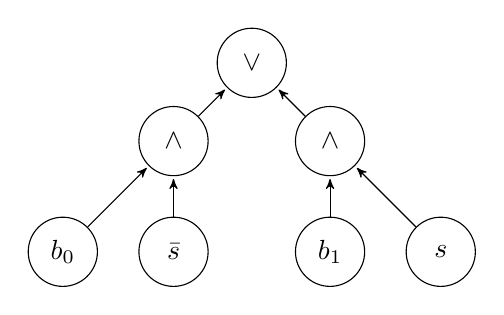
\begin{tikzpicture}[->, >=stealth', shorten >= 1pt, auto, node distance=4em, baseline=(current bounding box.center)]
		\node[state]	(or) 					{$\lor$};
		\node[state] 	(and0)[below left of=or]{$\land$};
		\node[state]	(and1)[below right of=or]{$\land$};
		\node[state]	(sbar)[below of=and0]{$\bar{s}$};
		\node[state]	(b0)[left of=sbar]{$b_0$};
		\node[state]	(b1)[below of=and1]{$b_1$};
		\node[state]	(s)[right of=b1]{$s$};
		\path 	
		(b0)	edge	node{} 	(and0)
		(sbar)	edge	node{}	(and0)
		(b1)	edge	node{} 	(and1)
		(s)		edge	node{}	(and1)
		(and0)	edge	node{}	(or)
		(and1)	edge	node{}	(or);
		\end{tikzpicture}
		\caption{Circuit for $\ff{MUX}(b_0, b_1, s)$. The output of the function is the value at the $\lor$ gate.}
		\label{fig:Mux}
	\end{figure}
	
	Recursively construct a depth $k$ tree of $\ff{MUX}$-gates. At the bottom are the bits $f_0, ..., f_{2^k-1}$. Above them are $2^{k-1}$ $\ff{MUX}$-gates labeled $\ff{MUX}_{k,0}, ..., \ff{MUX}_{k, 2^{k-1}-1}$ where 
	\[\ff{MUX}_{k,i} = \ff{MUX}(b_{f_{2i}}, b_{f_{2i + 1}}, \xor_{k}).\] 
	Level $j$ of the tree has $2^{j-1}$ $\ff{MUX}$-gates labeled with $\ff{MUX}_{j,0}, ..., \ff{MUX}_{j, 2^{j-1}-1}$ where 
	\[\ff{MUX}_{j,i} = (\ff{MUX}_{j+1,2i}, \ff{MUX}_{j+1,2i+1}, \xor_j)\] 
	for all $j \in [k]$. See Figure \ref{fig:MuxExample} for a small example.
	\begin{figure}[ht]
		\centering
		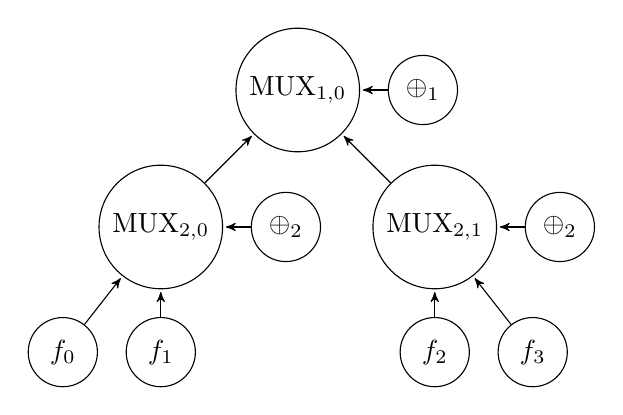
\begin{tikzpicture}[->, >=stealth', shorten >= 1pt, auto, node distance=7em, baseline=(current bounding box.center)]
		\node[state]	(mux10) 				{$\ff{MUX}_{1,0}$};
		\node[state]	(xor10) [right = 1em of mux10]{$\xor_1$};			
		\node[state]	(mux20) [below left of=mux10]{$\ff{MUX}_{2,0}$};
		\node[state]	(xor20) [right = 1em of mux20]{$\xor_2$};		
		\node[state]	(mux21) [below right of=mux10]{$\ff{MUX}_{2,1}$};
		\node[state]	(xor21) [right = 1em of mux21]{$\xor_2$};	
		\node[state]	(f1)	[below = 1em of mux20]{$f_1$};	
		\node[state]	(f0)	[left = 1em of f1]{$f_0$};	
		\node[state]	(f2)	[below = 1em of mux21]{$f_2$};	
		\node[state]	(f3)	[right = 1em of f2]{$f_3$};	
		\path 	
		(xor10)	edge	node{} 	(mux10)
		(xor20)	edge	node{}	(mux20)
		(xor21)	edge	node{} 	(mux21)
		(mux20)	edge	node{}	(mux10)
		(mux21)	edge	node{}	(mux10)
		(f0)	edge	node{}	(mux20)
		(f1)	edge	node{}	(mux20)
		(f2)	edge	node{}	(mux21)
		(f3)	edge	node{}	(mux21);
		\end{tikzpicture}
		\caption{Example of the constructed tree with $k = 2$.}
		\label{fig:MuxExample}
	\end{figure}
	
	There are $2^{k}$ leaves labeled by $f_0, ..., f_{2^{k}-1}$. Each of the $2^{k}-1$ $\ff{MUX}$-gates uses two $\xor_i$ sub-trees each containing $m$ leaves. This formula has $2^k + (2^{k}-1) \cdot 2m \in O(n^2/\log n)$ leaves. Thus $\leafsize_{B_2}(\ff{ANDREEV}_{k,m}) \in \Theta(n^2/\log n)$ with lower bound from the previous part.
\end{enumerate}
\vspace{1em}
\begin{problem}[LB Circuit Size of Monotone functions] Almost all monotone $n$-ary functions $f$ have DeMorgan circuits of size $\circuitsize(f) \in \Omega(2^n/n^{1.5})$.
\end{problem}
\begin{proof}
First we will show that there are at least $2^{\binom{n}{\floor{2/n}}}$ $n$-ary monotone functions. Consider the subsets of $[n]$ ordered by inclusion i.e. $\emptyset$ is at the bottom, $[n]$ is at the top, and an edge $(S_1, S_2)$ between $S_1, S_2 \subset [n]$ if $S_1 \subset S_2$. The family $\family{M}$ of all subsets containing $\floor{n/2}$ elements is an anti-chain of size $\binom{n}{\floor{n/2}}$. Consider maps $h: \family{M} \rightarrow \{0,1\}$. For each $h$, we can define a $n$-ary monotone function as follows. Let $M \in \family{M}$. If $h(M) = 0$, then for all proper supersets $M_{sup} \supset M$, $f(M_{sup}) = 1$. Otherwise if $h(M) = 1$, then for all proper subsets $M_{sub} \subset M$, $f(M_{sub}) = 0$. This defines a monotone function since the value of $f$ on a chain is monotonically increasing. Since there are  $2^{\binom{n}{\floor{n/2}}} = 2^{\Omega(2^n/\sqrt{n})}$ maps, there are at least this many $n$-ary monotone functions. 

Using the above and Shannon's lower bound for general $n$-ary Boolean functions, we can show that almost all monotone functions have DeMorgan circuit size $\Omega(2^n/n^{1.5})$. 

Let $s = 2^n/n^{1.5}$ and $A$ be the set of all circuits with size at most $s$. The set $B$ of monotone circuits of size at most $s$ is a subset of $A$. Note that $|A| \leq 2^{s}(s + 2n)^{2s}$ since each of the $s$ gates can be an $\land$ or $\lor$ and each gate can take two inputs from any of the $s$ gates or $2n$ literals. Further notice that any function $f$ with a circuit in $A$ also has $s!$ distinct circuits in $A$. Suppose $n \geq 22$ ($n^{1.5}> 100$). The number of monotone functions with circuit size at most $s$ is bounded above by
\[\frac{|B|}{s!} \leq \frac{|A|}{s!} \leq \frac{18^ss^{2s}}{\left(\frac{s}{e}\right)^s} \leq 50^ss^s \leq \left(\frac{50}{n^{1.5}}\right)^{2^n/n^{1.5}}2^{2^n/\sqrt{n}}\leq 2^{2^n/\sqrt{n} - 2^n/n^{1.5}}.\]
Thus at least $2^s$ monotone functions has circuit size greater than $s$.  
\end{proof}
\vspace{1em}
\begin{problem}[$\delta$-Approximate Majority] For $\delta \in (0,1/2)$, a $n$-ary Boolean functions $f$ is a $\delta$-approximate majority if for all $\vv{x} \in \{0,1\}^n$, 
	\begin{align*}
	\frac{|\vv{x}|}{n} \leq \frac{1}{2} - \delta &\implies f(\vv{x})= 0\\
	\frac{|\vv{x}|}{n} \geq \frac{1}{2} + \delta &\implies f(\vv{x})= 1\\
	\end{align*}
\end{problem}
Suppose $a, b, c$ are positive integers such that
\begin{equation}
	\label{eq:Q5Condition}
	\left(1 - \left(1 - \left(\frac{1}{2} - \delta\right)^a\right)^b\right)^c < 2^{-n} \mbox{ and } \left(1 - \left(1 - \left(\frac{1}{2} + \delta\right)^a\right)^b\right)^c > 1 - 2^{-n}.
\end{equation}
\begin{enumerate}
\item There exists $\Pi_3$ formulas of leafsize $abc$ that compute a $\delta$-approximate majority.
\begin{proof}
This will be similar to the proof that $\ff{MAJ}_n$ has poly-sized monotone formulas. In particular we will build a $\Pi_3$ formula with fan-in $c$, $b$, and $a$ respectively from top to bottom. Then populate the bottom-most level with values from a random projection.

Let $F$ be the formula as described above. The output of $F$ is a $\land$-gate, $t$, with fan-in $c$. The children of $t$ are $\lor$-gates, $r_1, ..., r_\gamma$ with fan-in $b$. The children of each $r_i$ are $\land$-gates $d_{i,1}, ..., d_{i,b}$ with fan-in $a$. The children of each gate $d_{i,j}$ are literals $y_{i,j,1}, ..., y_{i,j,a}$. Let the input to $F$ be $\vv{y} \in \{0,1\}^{abc}$, $\pi$ be a random projection from $\vv{y} \rightarrow \vv{x}$, and $F_{\pi}(\vv{x})$ be the formula with input $\pi(\vv{y})$. Let $A$ be the event that $F$ computes $\delta$-approximate majority. 

For $\pi$ such that $\pi(y_i)$ is chosen independently and uniformly from all elements of $\vv{x}$, we will show that $\Pr[A] > 1 - 2^{-n}$. Let $E_1$ and $E_2$ be the events $|\vv{x}|/n \leq \frac{1}{2} - \delta$ and $|\vv{x}|/n \geq 1/2 + \delta$ respectively. By conditioning, we have 
\[\Pr[A] = \Pr\left[F_{\pi}(\vv{x}) = 0 | E_1\right]\Pr\left[E_1\right] + \Pr\left[F_{\pi}(\vv{x}) = 1\middle|E_2\right]\Pr\left[E_2\right]\]
Since at most one of $\Pr[E_1] = 1$ or $\Pr[E_2] = 1$, we just need to show that both conditional probabilities on the RHS are bounded below by $1 - 2^{-n}$.

First condition on $E_1$ and let $p = \frac{1}{2} - \delta$. For any $d_{i,j}$, \[\Pr[d_{i,j}(\pi(y_{i,j,1}), ..., \pi(y_{i,j,a})) = 1| E_1] \leq \left(\frac{1}{2} - \delta\right)^{a}\]
since $\pi(y_{i,j,1}) \sim \bern(p)$. Similarly for any $r_i$, 
\[\Pr[r_{i}(d_{i,1}, ..., d_{i,b}) = 1|E_1] = 1 - \Pr[r_{i}(d_{i,1}, ..., d_{i,b}) = 0|E_1] \leq 1 - \left(1 - \left(\frac{1}{2} - \delta\right)^{\alpha}\right)^{b}.\]
Finally for $t$, 
\[\Pr[t(r_{1}, ..., r_{c}) = 1|E_1] \leq \left(1 - \left(1 - \left(\frac{1}{2} - \delta\right)^{\alpha}\right)^{b}\right)^{c}.\]
Together, with the inequalities given by the problem statement, we have 
\[\Pr[F_{\pi}(\vv{x}) = 0 | E_1] = 1 - \Pr[F_{\pi}(\vv{x}) = 1 | E_1] = 1 - \Pr[t(r_{1}, ..., r_{c}) = 1| E_1] > 1 - \frac{1}{2^{n}}.\]

Next condition on $E_2$ and let $p = \frac{1}{2} + \delta$. Using a similar argument, we have 
\begin{align*}
	\Pr\left[F_{\pi}(\vv{x}) = 1\middle|E_2\right] &= \Pr\left[t(r_1, ..., r_c) = 1\middle|E_2\right]\\
	&= \left(\Pr\left[r_i(d_{i,1}, ..., d_{i,b}) = 1| \middle|E_2\right]\right)^c\\
	&= \left(1 - \Pr\left[r_i(d_{i,1}, ..., d_{i,b}) = 0\middle|E_2\right]\right)^c\\
	&= \left(1 - \left(1 - \Pr\left[d_{i,j}(\pi(y_{i,j,1}), ..., \pi(y_{i,j,a})) = 1\middle|E_2\right]\right)^b\right)^c\\
	&\geq \left(1 - \left(1 - \left(\frac{1}{2} + \delta\right)^a\right)^b\right)^c\\
	&> 1 - 2^n
\end{align*}
so $\Pr[A] \geq 1 - 2^{-n}$ as required. Taking a union bound over all $2^n$ inputs, we see that there must exist some projection $\pi$ for which $F_{\pi}(\vv{x})$ is a $\delta$-approximate majority. Return the $\Pi_3$ formula obtained by hard-wiring $\pi$ into $F$.
\end{proof}

\item There are \emph{polynomial-sized} $\Pi_3$ formulas that compute a $\frac{1}{4}$-approximate majority\footnote{For all $d \geq 1$, there exists poly-sized $\Pi_{d+3}$ formulas that compute a $\frac{1}{(\log n)^d}$-approximate majority.}.

\emph{Solution.} Using the previous section, it suffices to take $\delta = 1/4$ and find $a,b,c$ which satisfy Equation (\ref{eq:Q5Condition}). From the upper bound we have 
\begin{align*}
	\left(1 - \left(1 - \left(\frac{1}{4}\right)^a\right)^b\right)^c &\leq \left(1 - \left(1 - \frac{b}{4^a}\right)\right)^c\\
	&\leq \left(\frac{b}{4^a}\right)^c\\ 
	&< \frac{1}{2^n}\\
\end{align*}
and from the lower bound we have
\begin{align*}
	\left(1 - \left(1 - \left(\frac{3}{4}\right)^a\right)^b\right)^c &\geq \left(1 - \exp\left(-b\left(\frac{3}{4}\right)^a\right)\right)^c\\
	&\geq 1 - c\exp\left(-b\left(\frac{3}{4}\right)^a\right)\\
	&> 1 - \frac{1}{2^n}.\\
\end{align*}
Together we require that $c\left(2a - \log b\right) > n$ and $b\left(3/4\right)^{a}\log e - \log c > n$. Choose $a = \log n$, $b = 2(4/3)^{a}\cdot n$, and $c = n$. Then, since $\log b = 1 + a\log \left(4/3\right) + \log n$,
\[c\left(2a - \log b\right) = n\log n \left(1 - \log \left(\frac{4}{3}\right) - \frac{1}{\log n}\right) \geq n\]
for sufficiently large $n$ such that $\log n > 3$ and $1 - \log \left(4/3\right) - (\log n)^{-1} > 1/3$. Further
\[b\left(3/4\right)^{a}\log e - \log c = 2n\log e - \log n > n.\]
Thus these values of $a$, $b$, and $c$ suffice, resulting in a $\Pi_3$ formula of leafsize 
\[abc = 2(4/3)^{\log n}n^2\log n \in O(n^3\log n)\] 
for $\frac{1}{4}$-approximate majority.
\end{enumerate}

\begin{comment}
\begin{problem}[UB Symmetric Functions] A \textbf{symmetric function} is an $n$-ary Boolean function $f$ whose values $f(\vv{x})$ only depending on the Hamming weight $|\vv{x}|$ of $\vv{x}$.
\end{problem}
\begin{enumerate}
\item (Warm-up) Let $f$ be an $n$-ary Boolean function where $f(\vv{x}) = 1 \iff |x|$ is congruent to one or three modulo five. Show that $f$ can be computed by DeMorgans circuits of size $O(n)$ and depth $O(\log n)$.
\begin{proof}
First we will show a constant depth circuit which takes two three bit numbers $x_2x_1x_0$ and $y_2y_1y_0$ less than five and outputs three bits $z_2z_1z_0$ which represents their sum modulo five. In particular each of $z_2$, $z_1$, and $z_0$ are represented by the following DNFs. Note that each clause has six literals but we only write the positive ones e.g. $x_2$ represented $x_2\bar{x}_1\bar{x}_0\bar{y}_2\bar{y}_2\bar{y}_0$.
\begin{align*}
z_2 &= x_2 \lor y_2 \lor x_1y_1 \lor x_0y_1y_0 \lor x_1x_0y_0\\
z_1 &= x_1x_0 \lor y_1y_0 \lor x_1 \lor y_1 \lor x_0y_0 \lor x_1y_0 \lor x_0y_1 \lor x_2y_1y_0 \lor x_1x_0y_2 \lor x_2y_2\\
z_0 &= x_0 \lor y_0 \lor x_1x_0 \lor y_1y_0 \lor x_2y_1 \lor x_1y_2 \lor x_1x_0y_1y_0 \lor x_2y_2.
\end{align*} 
We will prepend each input bit with two zeros so that the input to the circuit is of size $3n$. At each level, take pairs of three bits as input and output three bits. After $\log n$ levels, there will be three bits $t_2t_1t_0$ remaining. If $t_1t_0$ or $t_0$ then the circuit outputs one.   
\end{proof}
\item There exists DeMorgan circuits of \emph{constant-dept} which take three $n$-bit numbers $x$, $y$, and $z$ and outputs two $(n+1)$-bit number $u$ and $v$ such that $x + y + z = u + v$.
\begin{proof}
Let $x = \sum_{i=0}^{n-1}2^ix_i$, $y = \sum_{i=0}^{n-1}2^iy_i$, and $z = \sum_{i=0}^{n-1}2^iz_i$. Then let $u = \sum_{i=0}^{n}2^iu_i$ and $x = \sum_{i=0}^{n}2^iv_i$ where $u_n = 0$, $v_0 = 0$,
\[u_i = x_i \xor y_i \xor z_i \mbox{, and } v_{i+1} = x_i \land y_i \land z_i \mbox{ for } i \in \{0,...n-1\}.\]
Since we separated out the sum modulo two and the carry into $u$ and $v$ respectively, $x + y + z = u + v$ as require. Further the circuits needed to construct $u$ and $v$ are constant depth since we only need to xor a constant number of bits. 
\end{proof}
\item There exist DeMorgan circuits of depth $O(\log n)$ which take an input $\vv{x} \in \{0,1\}^n$ and outputs a $\ceil{\log n}$ bit number $u$ such that $u = |\vv{x}|$. 
\begin{proof}
Consider every bit in the input as a $1$-digit number. Construct a tree of $3$-to-$2$ addition gadgets as described in the previous part. Every level $i$ of the tree has two thirds as many number as level $i + 1$ and each number is longer by one bit. Thus, after $\log n$ levels, there will be a single output of length $\ceil{\log n}$.  
\end{proof}
\item Every symmetric function can be computed by DeMorgan circuits of size $O(n)$ and depth $O(\log n)$.

\emph{Solution.} By part 3 there exists a DeMorgan circuit $C$ of depth $O(\log n)$ which takes $n$ bits as input and outputs a $\ceil{\log n}$ bit number $u$ representing the hamming weight of $\vv{x}$. 

For every subset $S \subseteq [\ceil{\log n}]$ create an $\land$-gate representing the ``and'' of all variables with indices in $S$. This can be done recursively as follows: let $S_1, ..., S_{\ceil{\log n}}$ be the output of $C$. On the next level, let $S_{i_1,i_2} = S_{i_1} \land S_{i_2}$. Generally let $S_{i_1, ..., i_j} = S_{i_1, ..., i_{j-1}} \land S_{i_j}$. Finally take the $\lor$ of at most $n$ subsets $S$ representing numbers which satisfy the symmetric function. There $O(n)$ gates in $C$, $n$ gates representing the subsets of $[\ceil{\log n}]$, and $O(n)$ gates used to choose the satisfying numbers. Thus every symmetric function can be computed by a DeMorgan circuit of size $O(n)$ (and depth $O(\log n)$).
\end{enumerate}
\end{comment}
\addtocounter{problem}{1}
\newpage
\begin{problem}[UB $\class{AC}^0$ Circuit Size] Every $n$-ary Boolean function $f$ can be computed by an $\class{AC}^0$ circuit with $O(2^{n/2} \cdot n^c)$ gates for some constant $c$.
\end{problem}
\begin{proof}
Suppose $f$ is computed by DNF $F = C_1 \lor \cdots \lor C_k$ where the literals in each clause are arranged in lexicographical order. We will modify $F$ so that every clause has exactly $n$ literals. W.l.o.g suppose some clause $C_i = x_1 x_2 \cdots x_{t}$ has fewer than $n$ literals. Then we will remove $C_i$ from $F$ and add $2^{n-t}$ clauses with every possible combination of the variables $x_{t+1}, ..., x_{n}$ and their negation. For example, with $n = 4$, if $C_1 = x_1x_2$ then we will remove $C_1$ and add clauses $D_0 = x_1x_2\bar{x}_3\bar{x}_4$, $D_1 = x_1x_2\bar{x}_3x_4$, $D_2 = x_1x_2x_3\bar{x}_4$, and $D_3 = x_1x_2x_3x_4$. Let $F' = C_1' \lor \cdots \lor C_{k'}'$. Observe that $F(\vv{x}) = F'(\vv{x})$ for all inputs $\vv{x} \in \{0,1\}^n$.

Intuitively, the circuit divides the variables in-half and, for all settings of the first half which result in a satisfying assignment, checks to see if any of the matching second halves are satisfied.

Formally, we construct the following circuit $C$ from $F'$. Divide $[n]$ into two sets $A = \{1,..., n/2\}$ and $B = \{n/2 + 1, ..., n\}$ of size $n/2$ (we can assume that $n$ is even). Let $x_i^{1} \coloneqq x_i$ and $x_i^{0} \coloneqq \bar{x}_i$. For $\vv{b} \in \{0,1\}^B$, let 
\[\land_{\vv{b}} = \bigwedge_{j \in \vv{b}} x_{j}^{b_{j}}.\] 
For every $\vv{a} \in \{0,1\}^A$ define a $\land$-gate, $\pi_{\vv{a}}$, and a $\lor$-gate, $\sigma_{\vv{a}}$. Let $T_{\vv{a}} =  \{\vv{b}: F'(\vv{a}, \vv{b}) = 1\}$, then 
\[\pi_{\vv{a}} = \bigvee_{\vv{b} \in T_{\vv{a}}} \land_{\vv{b}} \mbox{ and } \sigma_{\vv{a}} = \left(\bigwedge_{i \in \vv{a}} x_i^{a_i}\right) \land \pi_{\vv{a}}.\]
Let $T = \{\vv{a}: \exists \vv{b} \in B \mbox{ such that } F(\vv{a}, \vv{b}) = 1\}$. The output of $C$ is $\lor_{\vv{a} \in T} \sigma_{\vv{a}}$.

Notice that $C$ is a depth four circuit. Further, since there are $2^{n/2}$ $\land_{\vv{b}}$ gates and two gates $\pi_{\vv{a}}$ and $\sigma_{\vv{a}}$ for each of the $2^{n/2}$ values of $\vv{a}$, $\circuitsize(F') \in O(2^{n/2})$ as required.   
\vspace{1em}
\begin{problem}[$\ff{MOD}_{p^k}$ for Prime $p$]
	The $n$-variable $\ff{MOD}_4$ function is computable by a polynomial-sized constant-depth $\class{AC}^0[2]$ circuit.
\end{problem}
\emph{Solution.}
Let the input to $\ff{MOD}_4$ be $\vv{x} \in \{0,1\}^n$ with entries $x_i$. Let gates $m_i = \ff{MOD}_2(x_1, ..., x_i)$ for $i \in [n]$ and gates $p_j = m_j \land m_{j+1}$ for $j \in [n-1]$. We claim that
\[\ff{MOD}_4(\vv{x}) = \overline{m}_n \land \ff{MOD}_2(m_1, ..., m_n, p_1, ..., p_{n-1}).\] 

To see why this is, consider the sequence $(m_1, ..., m_n)$. Divide this sequence into maximal blocks $b_1 \cdots b_k$ consisting of the same bit value. Let $k_0$ and $k_1$ be the number of $0$ and $1$ blocks respectively such that $k_0 + k_1 = k$. For example, 
\[(0,1,0,0,1,1,1,1,1,1,0) \implies b_1 = 0, b_2 = 1, b_3 = 00, b_4 = 111111, b_5 = 0\] 
$k_0 = 3$ and $k_1 = 2$. We claim that $\sum_{i = 1}^{n} x_i \equiv 0 \mod 4$ if and only if $k_1 \equiv 0 \mod 2$ and $m_n = 0$. First $\ff{MOD}_4(x_1, ..., x_n) = 0 \implies m_n = \ff{MOD}_2(x_1, ..., x_n) = 0$. Assuming that $m_n = 0$, consider a maximal block of consecutive ones $m_im_{i+1}\cdots m_{j}$ in the sequence. Since the block is maximal, $m_{i-1} = 0$ or $i = 1$ so there are an even number of ones among $x_1, ..., x_{i-1}$ and $x_i = 1$. Further $x_{i+1}, ..., x_{j} = 0$ since the parity $m_{i+1}, ..., m_{j}$ remains unchanged. Finally $m_{j+1} = 0$, since the block is maximal, so $x_{j+1} = 1$. Thus such a block of consecutive ones and the subsequent zero accounts for a pair of $1$s in the input. If there are an even number of pairs of $1$s, then $\sum_{i = 1}^{n} x_i \equiv 0 \mod 4$. 

It remains to show that $\ff{MOD}_2(m_1, ..., m_n, p_1, ..., p_{n-1})$ is equivalent to the parity of $k_1$ --- the number of maximal blocks of $1$s. Again suppose that $m_i\cdots m_{j}$ is a maximal block of $1$s. Observe that $p_i, p_{i+1} \cdots p_{j-1} = 1$. Thus 
\[\ff{MOD}_2(m_i, ..., m_{j}, p_i, ..., p_{j-1}) = \underbrace{1\xor\cdots \xor 1}_{2(j - i) + 1} = 1.\]
This is the case for all maximal blocks of $1$. Note that for all other $p_\ell$ such that $x_\ell = 0$ or $x_{\ell + 1} = 0$, $p_{\ell} = 0$. Since parity is a commutative operation, by grouping the $m_i$s and $p_i$s by maximal blocks of $1$s, $\ff{MOD}_2(m_1, ..., m_n, p_1, ..., p_{n-1})$ is exactly the parity of $k_1$. 

\end{proof}
% ===> END ASSIGNMENT
\end{document}